\documentclass{article} % Configuración del lenguaje. Reemplazar `english' por `spanish' para cambiar el idioma del documento.
\usepackage[spanish]{babel}
\usepackage[export]{adjustbox}
\usepackage{hyperref}
\usepackage{listings}
\lstset{language=[Sharp]C}
% Configuración del tamaño de página y márgenes. Reemplazar `letterpaper' por `a4paper' para el tamaño estándar del Reino Unido/UE.
\usepackage[letterpaper,top=2cm,bottom=2cm,left=3cm,right=3cm,marginparwidth=1.75cm]{geometry} 
% Paquetes útiles
\usepackage{amsmath} 
\usepackage{graphicx} 
\usepackage[colorlinks=true, allcolors=blue]{hyperref} 
\title{\textbf{Seminario Integrador:}
Ingeniería de software \newline Juegos Caribe}

\author{Leo Amaro \& Alfredo Montero :311 \\ Francisco Suárez Bellón :312} 
\begin{document} 
\maketitle 
\begin{abstract} 
En este seminario abordaremos el trabajo de las asignaturas Ingeniería de Software y Bases de Datos, el cual trata sobre la solución de la página web para los Juegos Caribe elaborado en el ambiente de .NET. 
\end{abstract}
 \section{Indroducción}
 \subsection{Alcance del producto}
    El alcance del producto abarca a todas las web que quieran mostrar competencias multideporte, su versatilidad le permite ser usado en otros escenarios donde haya un enfoque de equipos y enfrentamientos.

    Este producto se dirige a la competencia de los Juegos Caribes de la Universidad de la Habana. Su objetivo es de satisfacer a todo interesado en la competencia el estado actual de esta conociendo el medallero, asi como poder conocer el resultado de su facultad, equipo, composición o atleta de su preferencia.
\section{Descripción General}
\subsection{Funcionalidades del producto}
La función principal de este producto es de brindar la información del evento deportivo a todo interesado en esta con disponibilidad de conexion a internet
\begin{enumerate}

    \item Registrar las modalidades deportivas, Facultades y Atletas de la competencia.
    \item Actualizar los datos del estado actual de la competencia después de cada evento
    \item Brindar una sección de noticias relacionadas con cada evento deportivo
    \item Brindar de la información actualizada del estado de cada evento, modalidad, deporte, composición, equipo, atleta y facultad, su ranking en el medallero y su estado en la competencia.
    \item Realizar comentarios de las noticias 
    \item Poder actuar como moderador de los comentarios.
\end{enumerate}

\section{Características de los usuarios potenciales}
Debido a que los Juegos Caribe forman parte de los eventos 
de la Universidad de La Habana y están enfocados al cuerpo 
estudiantil de dicha institución, se considera a esta comunidad 
universitaria como usuarios potenciales de la página web.
Este usuario está comprendido en un rango etáreo que puede 
abarcar desde los 18 a los 26 años, incluyendo a aquellos estudiantes que sobrepasan los 23 años debido a cambios de 
carrera o que ya son egresados de la universidad y, según lo 
establecido en el Reglamento de los Juegos Caribe, pueden 
participar en el evento. 
Se caracterizan principalmente por un gran nivel de familiarización con las nuevas tecnologías, pues ellas forman parte 
del crecimiento y desenvolvimiento social de su generación. 
Asimismo, el usuario está interesado en conocer acerca de los 
partidos y torneos de los Juegos Caribe, además de conocer 
la puntuación de las facultades; por tanto, se convierte dicho 
interés en una de las misiones de la página.

\section{Análisis de referentes}
Con respecto al estudio de referentes, se pretendió analizar 
el comportamiento de las secciones y la visualidad en general 
de sitios webs vinculados a grandes eventos deportivos multidisciplinarios; no obstante, también se tomó como referencia 
los sitios webs reconocidos de distintos deportes, como es 
el caso de LaLiga, NBA, Roland Garros y MLB, para verificar 
cómo se administran las estadísticas de partidos, estados de 
competencia, noticias, fichas de equipos y perfiles de atletas.
Es por ello que el principal referente consultado para el diseño 
del sitio web de los Juegos Caribe fue la página de los Juegos 
Olímpicos, basándonos en la interfaz gráfica y presentación 
de los deportes de Tokyo 2020.

\section{Restricciones Generales}
\subsection{Restricciones del Cliente}
 El cliente ha expresado su preferencia por:
\begin{enumerate}
    \item Una interfaz de usuario intuitiva, la cuál ha sido brindada la plantilla por especialistas del ISDI.
    \item Un programa robusto que pueda aceptar el uso simultaneo de varios usuarios.
    \item Que sea independiente al lugar de desplieges asi como las condiciones de este.
\end{enumerate}
\subsection{Requerimientos de entorno }
 \begin{enumerate}
     \item Servidor con conexión estable a internet u otro medio de conexión local para el acceso de este.
     \item Maquina virtual Common Language Runtime (CLR) la cual pueda ejecutar código de Common Language Runtime (CLR): Lenguaje intermedio de .Net
     \item Estimado de un mínimo de 4gb de ram para la ejecución de este a bajo nivel de concurrencia.
     \item Personal encargado del manetenimiento y actualización de los datos.
 \end{enumerate}
\subsection{Requerimientos Funcionales}
\begin{enumerate}
    \item Disponibilidad de personal con responsabilidad de administrador, moderador y periodista por parte del cliente.
    \item Confianza absoluta del cliente por el personal de los roles anteriores.
    \item Información como el nombre de las facultades, deportes, modalidades, atletas, equipos , composiciones y eventos.
    
\end{enumerate}
 \section{Resumen}
 La plataforma está diseñada como una solución integral de gestión e infomación de datos. Para su desarrollo nos basamos en los principios de diseño y desarrollo solidos y metodoligía ágil garantizando seguridad y eficiencia.
 En el documento se abordarán los requerimientos funcionales, no funcionales y de entorno.
 
Enfoque en usabilidad y adaptabilidad a diferentes dispositivos.
Seguridad mediante autenticación basada en usuario - contraseña segura y
tokens JWT.
Uso de una variedad de tecnologías, incluyendo ASP.NET Core, Nextjs, y TypeScript, 
Compatibilidad del producto con una variedad de sistemas operativos y requisitos de
memoria RAM, CPU y espacio en disco recomendados.
Se presentarán las funcionalidades del producto usando un diagrama de casos de uso del
sistema.
Se justificará la selección de la metodología de desarrollo Scrum, con sprints de 2 semanas,
reuniones de SCRUM regulares, reuniones de retrospectiva y sprint review.
Se mostrará el uso de herramientas como "projects" de GitHub para el seguimiento del
progreso.
Se presentará un diagrama de la arquitectura escogida, que es la arquitectura limpia con
separación de responsabilidades, y se dirán las ventajas de su uso por las que se escogió para el
desarrollo del proyecto.
Se detallarán los patrones de repositorio y unidad de trabajo para acceso a datos que fueron
elegidos para la realización del proyecto.
Se verán los principios de diseño que se aplican, como SOLID, YAGNI (You Aren't Gonna Need It) y
KISS (Keep It Simple, Stupid) para mantener la simplicidad y evitar la implementación de
características innecesarias.
Al final se presentará el modelo que determina la estructura de la base de datos del proyecto.


\section{Seguridad}
\subsection*{Confidencialidad} 
Los datos solo pueden ser modificados por usuarios con identidad y contraseña debidamente guardada, los cuales su asignación en cada rol queda del lado del cliente. Se ha confirmado por parte del cliente que el modelo jerárquico propuesto satisface sus condiciones y que es de su cargo la confianza en ellos, especialmente en el administrador. 


\begin{lstlisting}
public class Usuario
{
    public int Id { get; set; }
    public string NombreUsuario { get; set; }
    public string ContrasenaHash { get; set; }
    public string Rol { get; set; }
    // Otras propiedades
}

// Funcion para verificar las credenciales de un usuario
public bool VerificarCredenciales(string nombreUsuario, string contrasena)
{
    // Buscar al usuario en la base de datos por nombre de usuario
    var usuario = _dbContext.Usuarios.FirstOrDefault(u => u.NombreUsuario == nombreUsuario);
    if (usuario != null)
    {
        // Verificar la contrase~na utilizando el hash almacenado
        var contrase~naHashIngresada = CalcularHashContrasena(contrasena, usuario.NombreUsuario);
        return usuario.ContrasenaHash == contrasenaHashIngresada;
    }
    return false;
}

// Funcion para calcular el hash de la contrasena
    public string CalcularHashContrasena(string contrasena, string salt)
{
    using (var sha256 = SHA256.Create())
    {
        var contrasenaSalted = contrasena + salt;
        var hashBytes = sha256.ComputeHash(Encoding.UTF8.GetBytes(contrasenaSalted));
        return BitConverter.ToString(hashBytes).Replace("-", "").ToLower();
    }
}


\end{lstlisting}
\begin{enumerate}
    \item Uso de encriptación de contraseñas mediante Hash sha256
    \item Comprobación del usuario por su id y contraseña
    
\end{enumerate}

Validación mediante JWT:
\begin{lstlisting}
    public class JwtService
{
    private readonly string _secretKey;

    public JwtService(string secretKey)
    {
        _secretKey = secretKey;
    }

    public string GenerateToken(string username, int userId)
    {
        var tokenHandler = new JwtSecurityTokenHandler();
        var key = Encoding.ASCII.GetBytes(_secretKey);

        var tokenDescriptor = new SecurityTokenDescriptor
        {
            Subject = new ClaimsIdentity(new Claim[]
            {
                new Claim(ClaimTypes.Name, username),
                new Claim(ClaimTypes.NameIdentifier, userId.ToString())
            }),
            Expires = DateTime.UtcNow.AddDays(7),
            SigningCredentials = new SigningCredentials(new SymmetricSecurityKey(key), SecurityAlgorithms.HmacSha256Signature)
        };

        var token = tokenHandler.CreateToken(tokenDescriptor);
        return tokenHandler.WriteToken(token);
    }

    public ClaimsPrincipal ValidateToken(string token)
    {
        var tokenHandler = new JwtSecurityTokenHandler();
        var key = Encoding.ASCII.GetBytes(_secretKey);

        try
        {
            tokenHandler.ValidateToken(token, new TokenValidationParameters
            {
                ValidateIssuerSigningKey = true,
                IssuerSigningKey = new SymmetricSecurityKey(key),
                ValidateIssuer = false,
                ValidateAudience = false,
                ClockSkew = TimeSpan.Zero
            }, out var validatedToken);

            return validatedToken?.Principal;
        }
        catch
        {
            return null;
        }
    }
}
\end{lstlisting}
\begin{enumerate}
    \item Los tokens JWT se usarán para autorizar a los usuarios a acceder a recursos específicos
de la aplicación web dependiendo de su rol.
\item Los tokens JWT se firmán digitalmente con una clave secreta (guardada como variable de entorno). Esto ayuda a proteger los
datos del usuario.

\end{enumerate}
\subsection{Integridad}
\begin{enumerate}
    \item Mediante el control de sesiones se garantiza la integridad del programa, protegiendo de la corrupción de datos.
    \item Mediante el uso de moderadores de comentarios se dispondrá de un filtro sobre comentarios no deseados o acordes con las políticas del cliente.
\end{enumerate}
\subsection{Disponibilidad}
 Garantizaremos la capacidad de nuestra aplicación para proporcionar
acceso a los datos y servicios cuando se necesita mediante la implementación eficiente,
dentro del alcance posible, de las solicitudes al servidor y consultas a la base de datos. Para
esto tendremos en cuenta las siguientes técnicas:
\begin{enumerate}
    \item El desarrollos sobre entornos pensado para la portabilidad de este, robusto y con años de confianza por parte de la comunidad
    \item Optimización del código, la cual asegura que el código de la aplicación web esté bien escrito y
optimizado para el rendimiento.
\item Utilización de un almacenamiento de datos eficiente asi como un ORM robusto y eficiente.
\item Consultas ligeras: Evitar hacer consultas que requieran una gran cantidad de datos.
Limitar las consultas a los datos que son realmente necesarios.
\item La tolerancia a fallos: Implementar mecanismos para que la aplicación pueda
recuperarse de fallos.

\end{enumerate}

\section{Funcionalidades del producto}
  \subsection{Story Board}
         \includegraphics[width=\textwidth, max height=\textheight, keepaspectratio]{OIG (1).jpeg}
         
         \subsection{Diagrama de descripción de actores}
         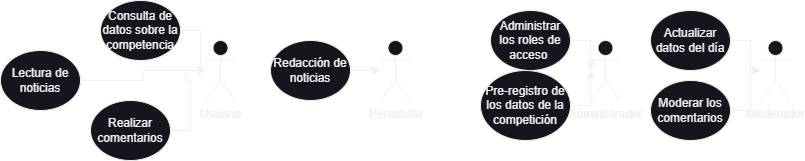
\includegraphics[width=\textwidth, max height=\textheight, keepaspectratio]{Diagrama de descripcion de actores actualizado.png}
         En el diagrama de descripción anterior se muestran los roles de cada actor.
    \subsection{Descripción de roles}
    \begin{enumerate}
    %USuario comun
        \item \textbf{Usuario Común:} Este tipo de usuario no necesita verificación y puede realizar las siguientes
    acciones:
 \begin{enumerate}
     \item  Navegar por la página principal de la plataforma.
     \item Acceder a la información de los deportes
     \item Realizar búsquedas específicas de deportes o equipo
 \end{enumerate}
%Administrador
\item \textbf{Administrador:} Este tipo de usuario tiene acceso a todas las funcionalidades de la plataforma y
puede realizar cualquier tipo de acción.
%Periodista
\item \textbf{Periodista: }Este tipo de usuario tiene acceso a una sección específica en la página web donde
puede insertar noticias relacionadas con los deportes. Esta sección solo es visible para el periodista
y el administrador.
%moderador 
\item \textbf{Moderador:}  Este tipo de usuario se encarga de insertar los resultados de los partidos y la información relacionada con los mismos.



    \end{enumerate}

\section{Enfoque Metodológico}
Se decidió utilizar Scrum porque es una metodología ágil que puede ser muy beneficiosa para el
desarrollo del proyecto por varias razones:
\begin{enumerate}
    \item \textbf{Iteraciones cortas y entregas frecuentes:}  Scrum se basa en sprints, que son períodos de
tiempo cortos (en nuestro caso 2 semanas) durante los cuales se completa un conjunto
definido de tareas, lo que tiende a aumentar la productividad y la concentración. También
permite proporcionar actualizaciones frecuentes y tangibles a las partes interesadas, lo que
puede ser especialmente útil en un mercado en constante cambio como el de las agencias de
viajes.
\item \textbf{Adaptabilidad:} Dado que Scrum se basa en la inspección y adaptación constantes, podemos
ajustar rápidamente los planes y prioridades en respuesta a los cambios en los requisitos del
negocio.
\item \textbf{Enfoque en el valor del negocio:} En Scrum, las tareas se priorizan en función de su valor
para el negocio. Esto asegura que estemos siempre trabajando en las características que
proporcionarán el mayor valor a los clientes.
\item \textbf{Transparencia:} Scrum proporciona una visibilidad clara del progreso del proyecto a todas
las partes interesadas a través de sus artefactos (como el backlog del producto y el gráfico de
burndown) y ceremonias (como la planificación del sprint y la revisión del sprint).
\item \textbf{Colaboración y comunicación mejoradas:}  Scrum fomenta la colaboración y la
comunicación abierta entre los miembros del equipo y las partes interesadas. Esto puede ser
especialmente beneficioso porque nuestro equipo está compuesto por personas con
diferentes habilidades y antecedentes.
\end{enumerate}

Impelementación de la Metodología:
\begin{enumerate}
    \item \textbf{Duración de los Sprints:} 10 diás cada uno.
    \item \textbf{Frecuencia de las reuniones( SCRUM o Stand-up):} Martes y Viernes. Esta programación nos brinda una visión actualizada del avance del proyecto y permite abordar cualquier dificultad.
    \item \textbf{. Reuniones de Retrospectiva y Sprint Review:} Domingos. Nos permite evaluar el desempeño del equipo y pudiendo programar ajustes futuros.
    \item \textbf{Herramientas de Control del Progreso:} Se utilizan varias vías:
    %Enumerador de COntrol de progreso
    \begin{enumerate}
        \item \textbf{Github Projects} para tener compartido el  RoadMap, además poder seleccionar las tareas a terminar. 
        \newline
        \includegraphics[width=\textwidth, max height=\textheight, keepaspectratio]{photo_2023-11-04_16-51-14.jpg}
        
        \item \textbf{Grupo en telegram} con división y pignorado de mensajes según el debate. 
        \item \textbf{Code With Me} de JetBrains para la programación colaborativa en tiempo real
    \end{enumerate}
\end{enumerate}
\section{Arquitectura}
%Modificar aca
La Arquitectura Limpia también es una opción sólida para el desarrollo de una página web que muestre resultados de una competencia, ya que se caracteriza por su alta modularidad y separación de responsabilidades, lo que la hace especialmente adecuada para aplicaciones web empresariales y escalables.

A continuación se presentan algunos de los beneficios clave de la Arquitectura Limpia:

\begin{itemize}
    \item Separación de Responsabilidades: La Arquitectura Limpia divide claramente la aplicación en capas y componentes, lo que facilita la comprensión y el mantenimiento del código. Esto es crucial en aplicaciones empresariales, donde se espera que el código sea escalable y fácil de mantener.
    \item Independencia de la Infraestructura: La Arquitectura Limpia separa la lógica de negocio de la infraestructura, lo que significa que la lógica empresarial no depende de frameworks o tecnologías específicas. Esto permite cambiar la tecnología subyacente sin afectar la funcionalidad principal de la aplicación.
    \item Testabilidad: La separación de responsabilidades y la independencia de la infraestructura facilitan la escritura de pruebas unitarias y de integración. Esto es esencial para garantizar la calidad del software y la detección temprana de errores.
    \item Escalabilidad: La modularidad de la Arquitectura Limpia permite escalar componentes de manera individual. Puedes escalar la capa de presentación, la capa de aplicación y la capa de dominio según sea necesario sin afectar otras partes de la aplicación.
    \item Reutilización de Código: La claridad en la separación de responsabilidades y la independencia de la infraestructura promueve la reutilización del código en diferentes partes de la aplicación, lo que ahorra tiempo y esfuerzo en el desarrollo.
\end{itemize}

 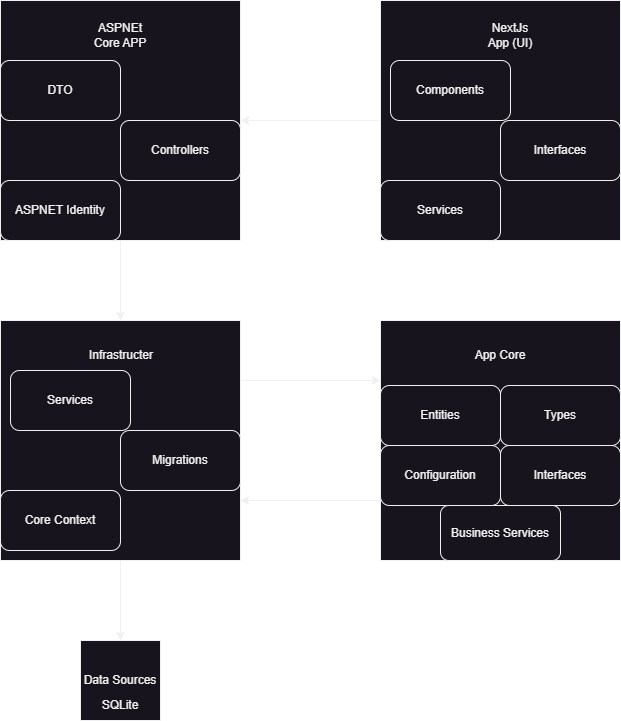
\includegraphics[width=\textwidth, max height=\textheight, keepaspectratio]{arquitectoraaa.png}
 \newline
  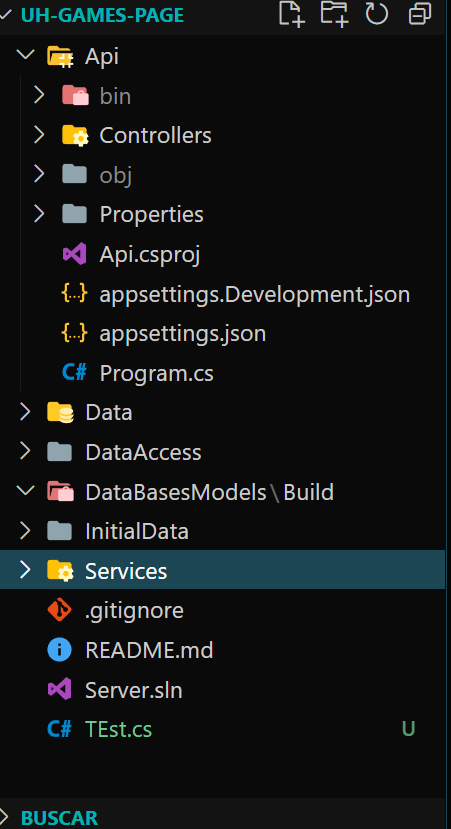
\includegraphics[width=\textwidth, max height=\textheight, keepaspectratio]{Captura de pantalla 2023-11-04 171245.png}

\section{Patrones}
La implementación de la Arquitectura Limpia en el desarrollo de una aplicación web para mostrar los resultados de una competencia es una opción sólida que se basa en varios principios de diseño SOLID. Se utilizará el patrón Repositorio para abstraer y gestionar las operaciones de acceso a datos de una manera más estructurada y facilitar la reutilización del código en toda la aplicación. Se creará una capa de acceso a datos que contendrá una serie de repositorios personalizados, cada uno actuando como una capa de abstracción sobre el DbContext de Entity Framework y utilizando métodos proporcionados por EF para llevar a cabo las operaciones de lectura y escritura. La clase DbContext será el punto central para administrar la conexión a la base de datos y las transacciones, rastreando las entidades, realizando seguimiento de los cambios y administrando la comunicación con la base de datos.

Se aplicarán los siguientes principios de diseño SOLID:

\begin{itemize}
    \item Principio de responsabilidad única: Se descompondrán las clases y módulos en unidades lógicas, cada una con una única responsabilidad. Esto permitirá modificar o extender una funcionalidad sin afectar otras partes del sistema.
    \item Principio de abierto/cerrado: La aplicación web permitirá la extensión de funcionalidades sin modificar el código existente. Se utilizarán la herencia, interfaces y patrones de diseño para agregar nuevas características o servicios sin alterar las clases existentes, asegurando que la aplicación sea fácilmente adaptable a futuras mejoras.
    \item Principio de sustitución de Liskov: Se garantizará que las subclases hereden y extiendan el comportamiento de las superclases de manera coherente y predecible, sin romper la funcionalidad del sistema.
    \item Principio de segregación de interfaces: Se dividirán las interfaces en conjuntos más pequeños y específicos, evitando que las clases implementen métodos que no son relevantes para su funcionalidad y permitiendo una mejor organización del código.
    \item Principio de inversión de dependencias: Las clases de alto nivel dependerán de abstracciones en lugar de implementaciones concretas, proporcionando flexibilidad y permitiendo cambiar las implementaciones concretas sin afectar a los módulos de alto nivel.
\end{itemize}

Además, se adoptarán los principios YAGNI (You Aren't Gonna Need It) y KISS (Keep It Simple, Stupid) en el diseño de la aplicación. Se centrará en proporcionar las capacidades esenciales que los usuarios necesitarán para utilizar la aplicación de manera efectiva desde el principio, evitando la implementación de funcionalidades no necesarias en este momento. Se mantendrá una interfaz de usuario simple y fácil de navegar, lo que se traducirá en un diseño limpio y una estructura intuitiva que permitirá a los usuarios encontrar y utilizar las funcionalidades de la aplicación de manera eficiente. Se evitará la incorporación de características innecesariamente complejas o detalles superfluos en la aplicación, lo que se traducirá en un código más limpio y fácil de mantener.

%%%Insertar lo de Cruddddddd

\section{Modelo de Base de Datos}
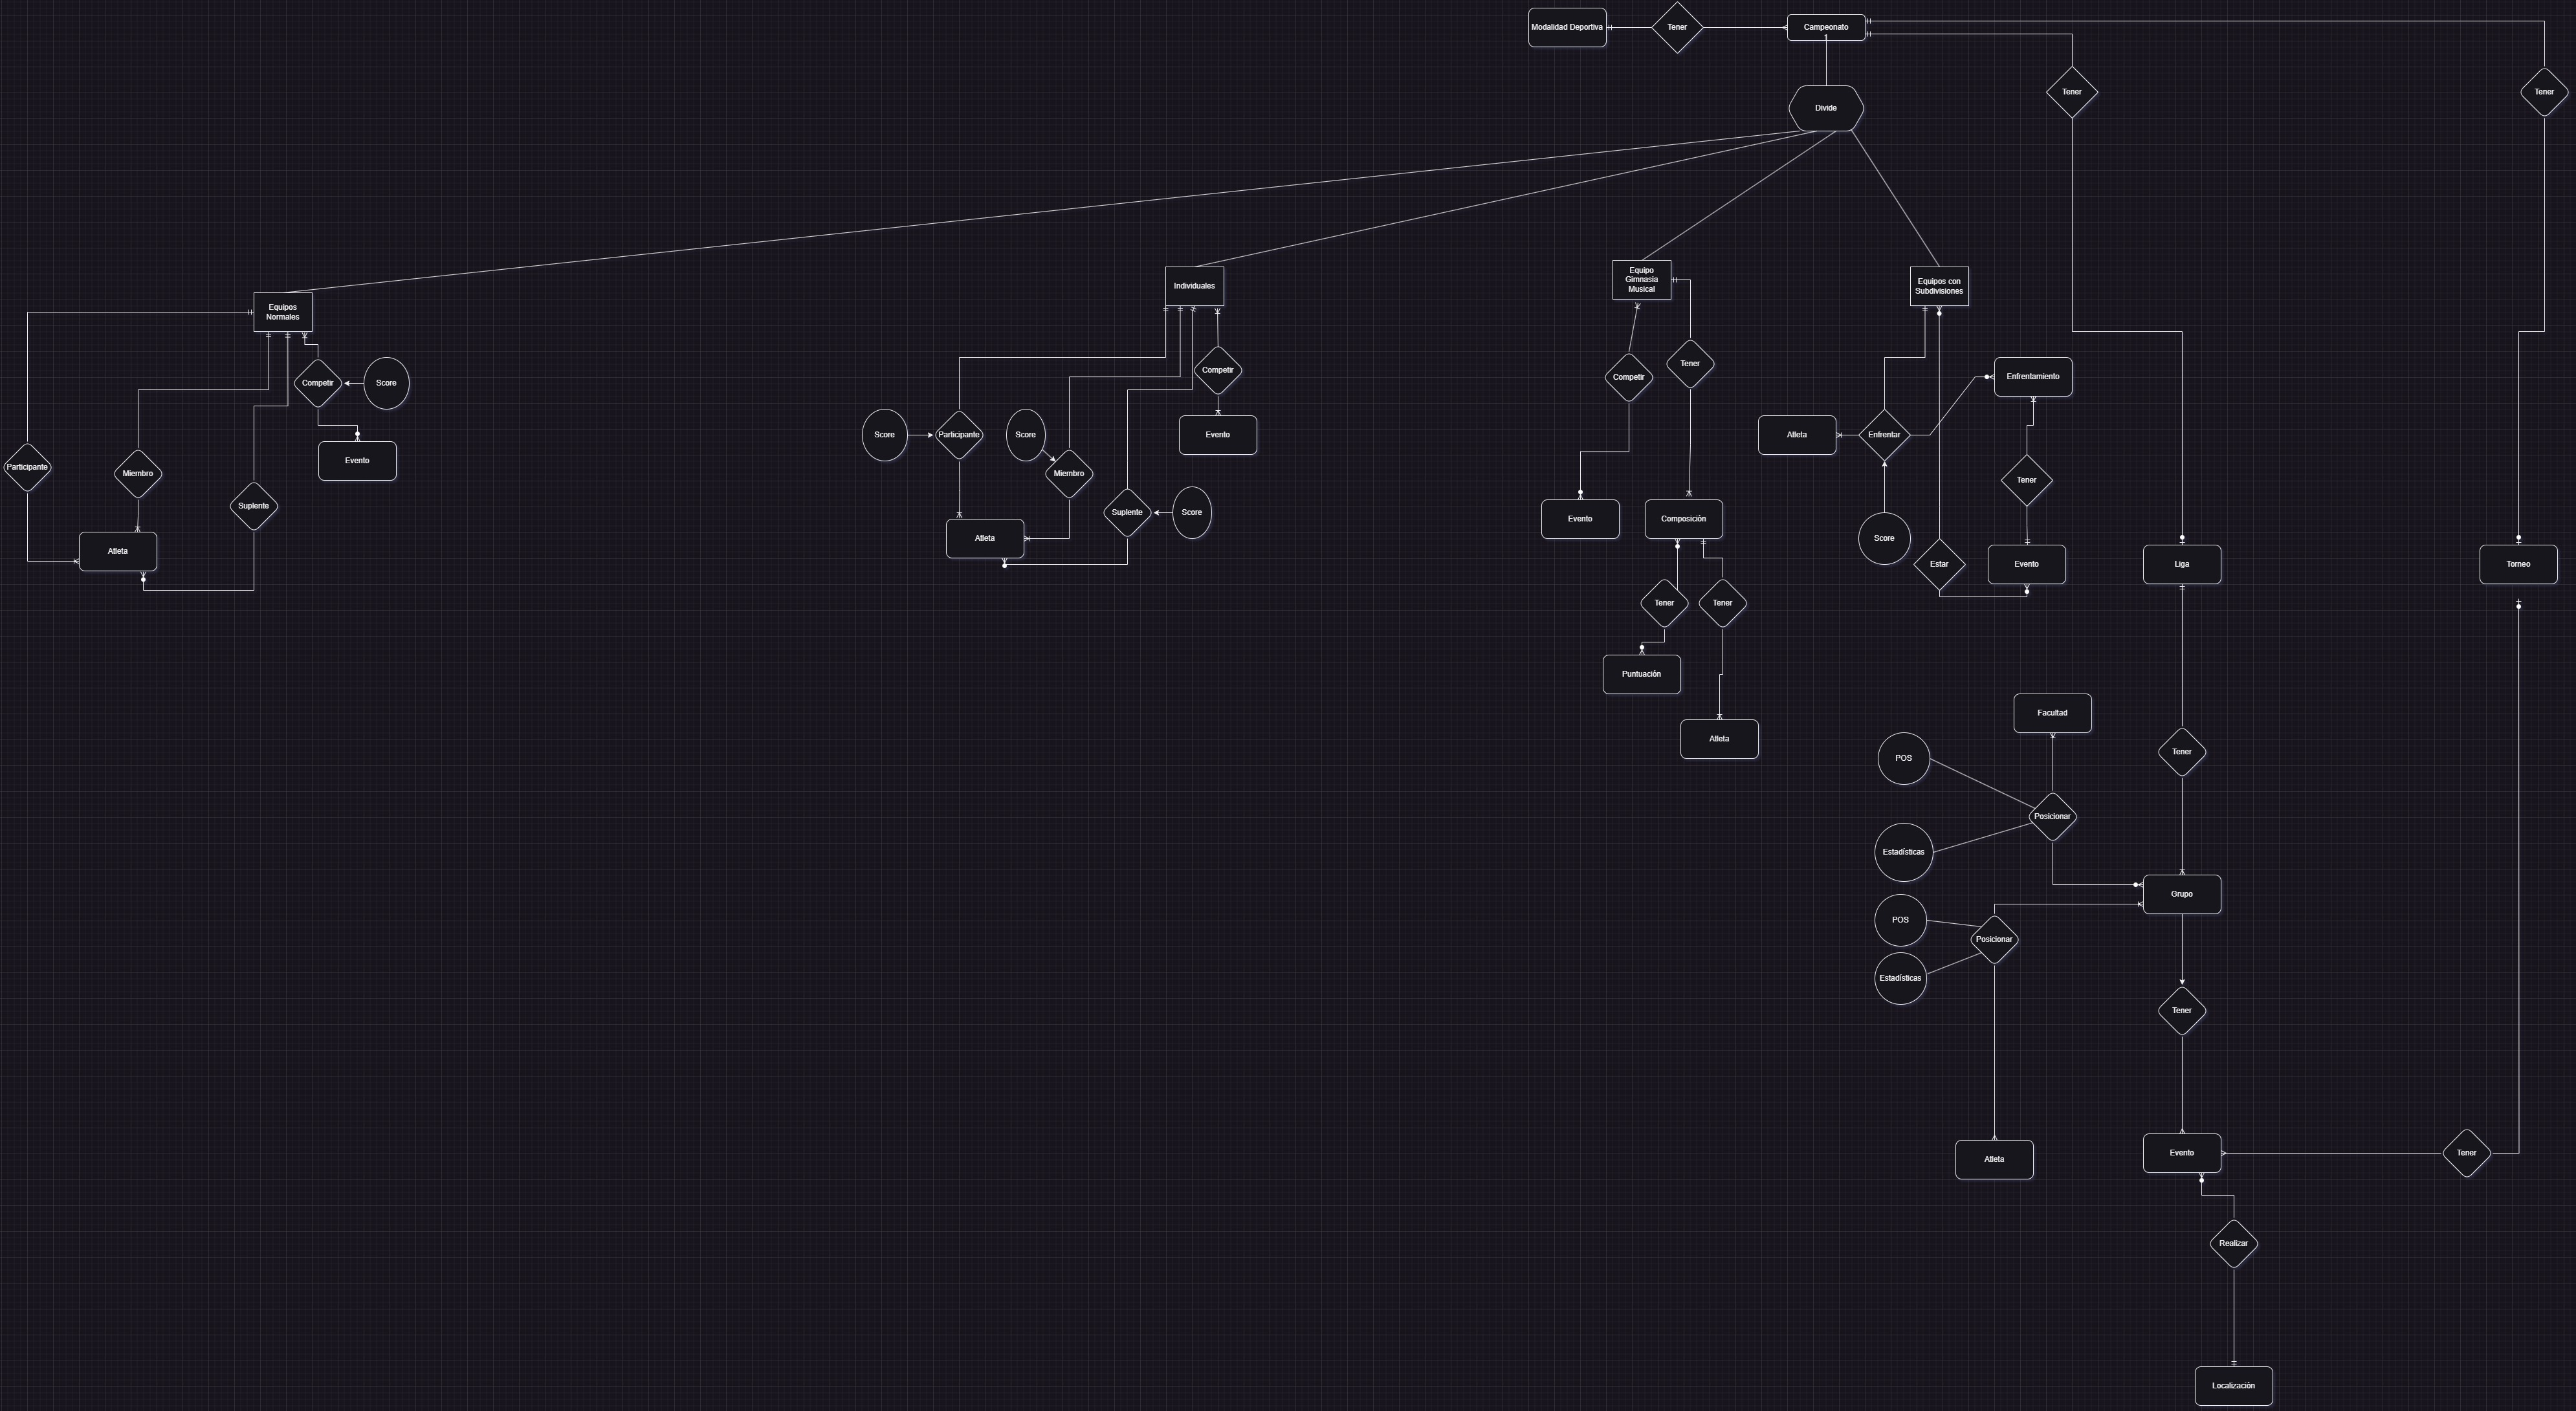
\includegraphics[width=\textwidth, max height=\textheight, keepaspectratio]{Caribes_General.jpg}
\subsection{Implementación}
Se utiliza una base de datos relacional: SQLite la cual por su versatilidad y  facilidad de configuración y uso de recursos ha sido la adecuada para este proyecto.
Se ha realizado el desarrollo del modelo de esta y su integración con el resto de la API se ha realizado mediante EntityFramework, ORM el cual nos permite con eficiencia relizar la creación de la misma desde un modelo de clases y poder hacer migraciones automaticas, ademas del uso de las consulta LINQ 
\newline
\includegraphics[width=\textwidth, max height=\textheight, keepaspectratio]{tabla q.png}
\end{document}
